\begin{figure}[H]
	\centering
	\caption{Alongamento de uma fibra.}
	\vspace*{5mm}
	\tikzset{every picture/.style={line width=0.75pt}} %set default line width to 0.75pt        

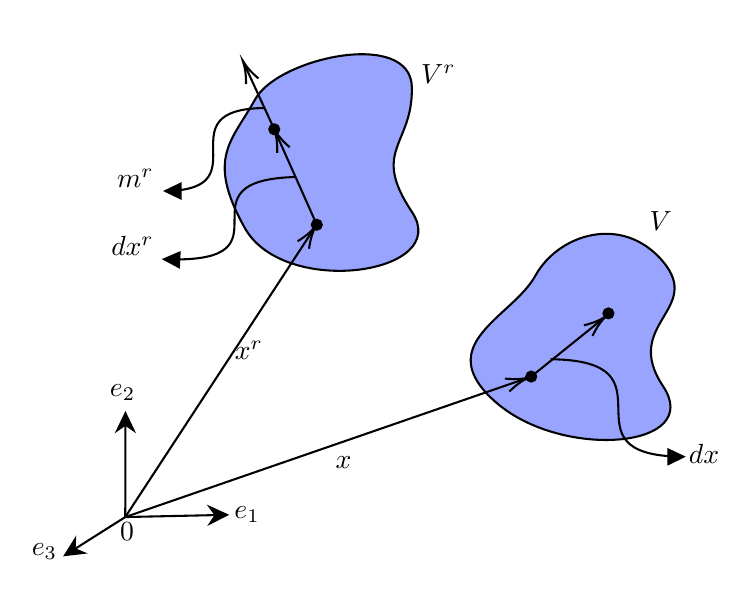
\begin{tikzpicture}[x=0.75pt,y=0.75pt,yscale=-1,xscale=1]
%uncomment if require: \path (0,300); %set diagram left start at 0, and has height of 300

%Shape: Polygon Curved [id:ds1267896810110165] 
\draw  [fill={rgb, 255:red, 0; green, 27; blue, 255 }  ,fill opacity=0.4 ] (447.5,126) .. controls (458.5,106) and (489.5,96) .. (509,119.2) .. controls (528.5,142.4) and (489,149.2) .. (509,179.2) .. controls (529,209.2) and (460.5,215) .. (428.5,187) .. controls (396.5,159) and (436.5,146) .. (447.5,126) -- cycle ;
%Shape: Polygon Curved [id:ds6304398480649873] 
\draw  [fill={rgb, 255:red, 0; green, 27; blue, 255 }  ,fill opacity=0.4 ] (312.5,41) .. controls (323.5,21) and (387.5,7) .. (388,35.2) .. controls (388.5,63.4) and (368,65.2) .. (388,95.2) .. controls (408,125.2) and (326.5,137) .. (307.5,103) .. controls (288.5,69) and (301.5,61) .. (312.5,41) -- cycle ;
%Straight Lines [id:da3839595512989218] 
\draw    (249.92,242.28) -- (340.59,103.73) ;
\draw [shift={(341.69,102.06)}, rotate = 483.2] [color={rgb, 255:red, 0; green, 0; blue, 0 }  ][line width=0.75]    (10.93,-3.29) .. controls (6.95,-1.4) and (3.31,-0.3) .. (0,0) .. controls (3.31,0.3) and (6.95,1.4) .. (10.93,3.29)   ;
%Straight Lines [id:da17029354313067024] 
\draw    (249.92,242.28) -- (442.37,175.74) ;
\draw [shift={(444.26,175.09)}, rotate = 520.9300000000001] [color={rgb, 255:red, 0; green, 0; blue, 0 }  ][line width=0.75]    (10.93,-3.29) .. controls (6.95,-1.4) and (3.31,-0.3) .. (0,0) .. controls (3.31,0.3) and (6.95,1.4) .. (10.93,3.29)   ;
%Shape: Circle [id:dp9281208088104935] 
\draw  [fill={rgb, 255:red, 0; green, 0; blue, 0 }  ,fill opacity=1 ] (339.8,101.45) .. controls (339.8,100.12) and (340.87,99.05) .. (342.2,99.05) .. controls (343.53,99.05) and (344.6,100.12) .. (344.6,101.45) .. controls (344.6,102.78) and (343.53,103.85) .. (342.2,103.85) .. controls (340.87,103.85) and (339.8,102.78) .. (339.8,101.45) -- cycle ;
%Shape: Circle [id:dp6936122735823536] 
\draw  [fill={rgb, 255:red, 0; green, 0; blue, 0 }  ,fill opacity=1 ] (443.1,174.6) .. controls (443.1,173.27) and (444.17,172.2) .. (445.5,172.2) .. controls (446.83,172.2) and (447.9,173.27) .. (447.9,174.6) .. controls (447.9,175.93) and (446.83,177) .. (445.5,177) .. controls (444.17,177) and (443.1,175.93) .. (443.1,174.6) -- cycle ;
%Straight Lines [id:da8900818525972407] 
\draw    (249.92,242.28) -- (250,194.2) ;
\draw [shift={(250,191.2)}, rotate = 450.09] [fill={rgb, 255:red, 0; green, 0; blue, 0 }  ][line width=0.08]  [draw opacity=0] (10.72,-5.15) -- (0,0) -- (10.72,5.15) -- (7.12,0) -- cycle    ;
%Straight Lines [id:da3194428698841316] 
\draw    (249.92,242.28) -- (297,241.26) ;
\draw [shift={(300,241.2)}, rotate = 538.76] [fill={rgb, 255:red, 0; green, 0; blue, 0 }  ][line width=0.08]  [draw opacity=0] (10.72,-5.15) -- (0,0) -- (10.72,5.15) -- (7.12,0) -- cycle    ;
%Straight Lines [id:da7047854692062743] 
\draw    (249.92,242.28) -- (222.54,259.6) ;
\draw [shift={(220,261.2)}, rotate = 327.69] [fill={rgb, 255:red, 0; green, 0; blue, 0 }  ][line width=0.08]  [draw opacity=0] (10.72,-5.15) -- (0,0) -- (10.72,5.15) -- (7.12,0) -- cycle    ;
%Straight Lines [id:da6597397687420881] 
\draw    (445.5,174.6) -- (479.9,146.86) ;
\draw [shift={(481.46,145.6)}, rotate = 501.11] [color={rgb, 255:red, 0; green, 0; blue, 0 }  ][line width=0.75]    (10.93,-3.29) .. controls (6.95,-1.4) and (3.31,-0.3) .. (0,0) .. controls (3.31,0.3) and (6.95,1.4) .. (10.93,3.29)   ;
%Curve Lines [id:da14263489472034885] 
\draw    (454.9,166.25) .. controls (517.94,166.91) and (457.92,212.11) .. (517.21,213.18) ;
\draw [shift={(520,213.2)}, rotate = 539.73] [fill={rgb, 255:red, 0; green, 0; blue, 0 }  ][line width=0.08]  [draw opacity=0] (8.93,-4.29) -- (0,0) -- (8.93,4.29) -- cycle    ;
%Straight Lines [id:da07035536989410152] 
\draw    (342.2,101.45) -- (322.51,57.28) ;
\draw [shift={(321.7,55.45)}, rotate = 425.98] [color={rgb, 255:red, 0; green, 0; blue, 0 }  ][line width=0.75]    (10.93,-3.29) .. controls (6.95,-1.4) and (3.31,-0.3) .. (0,0) .. controls (3.31,0.3) and (6.95,1.4) .. (10.93,3.29)   ;
%Curve Lines [id:da028710661205021193] 
\draw [color={rgb, 255:red, 0; green, 0; blue, 0 }  ,draw opacity=1 ]   (331.95,78.45) .. controls (272.41,79.98) and (333.61,119.78) .. (270.47,118.11) ;
\draw [shift={(267.5,118)}, rotate = 362.53] [fill={rgb, 255:red, 0; green, 0; blue, 0 }  ,fill opacity=1 ][line width=0.08]  [draw opacity=0] (8.93,-4.29) -- (0,0) -- (8.93,4.29) -- cycle    ;
%Shape: Circle [id:dp7331203369042449] 
\draw  [fill={rgb, 255:red, 0; green, 0; blue, 0 }  ,fill opacity=1 ] (319.3,55.45) .. controls (319.3,54.12) and (320.37,53.05) .. (321.7,53.05) .. controls (323.03,53.05) and (324.1,54.12) .. (324.1,55.45) .. controls (324.1,56.78) and (323.03,57.85) .. (321.7,57.85) .. controls (320.37,57.85) and (319.3,56.78) .. (319.3,55.45) -- cycle ;
%Shape: Circle [id:dp9204751236184672] 
\draw  [fill={rgb, 255:red, 0; green, 0; blue, 0 }  ,fill opacity=1 ] (480.3,144.15) .. controls (480.3,142.82) and (481.37,141.75) .. (482.7,141.75) .. controls (484.03,141.75) and (485.1,142.82) .. (485.1,144.15) .. controls (485.1,145.48) and (484.03,146.55) .. (482.7,146.55) .. controls (481.37,146.55) and (480.3,145.48) .. (480.3,144.15) -- cycle ;
%Straight Lines [id:da33979219300798014] 
\draw    (307.35,24.22) -- (321.7,55.45) ;
\draw [shift={(306.52,22.4)}, rotate = 65.33] [color={rgb, 255:red, 0; green, 0; blue, 0 }  ][line width=0.75]    (10.93,-3.29) .. controls (6.95,-1.4) and (3.31,-0.3) .. (0,0) .. controls (3.31,0.3) and (6.95,1.4) .. (10.93,3.29)   ;
%Curve Lines [id:da3062989434683383] 
\draw [color={rgb, 255:red, 0; green, 0; blue, 0 }  ,draw opacity=1 ]   (317.32,45.2) .. controls (267.93,45.59) and (315.34,83.63) .. (270.95,85.15) ;
\draw [shift={(268.12,85.2)}, rotate = 360] [fill={rgb, 255:red, 0; green, 0; blue, 0 }  ,fill opacity=1 ][line width=0.08]  [draw opacity=0] (8.93,-4.29) -- (0,0) -- (8.93,4.29) -- cycle    ;

% Text Node
\draw (301,235.6) node [anchor=north west][inner sep=0.75pt]    {$\vt{e}_{1}$};
% Text Node
\draw (349.71,211.84) node [anchor=north west][inner sep=0.75pt]    {$\vt{x}$};
% Text Node
\draw (301.21,156.24) node [anchor=north west][inner sep=0.75pt]    {$\vt{x}^{r}$};
% Text Node
\draw (391,22.6) node [anchor=north west][inner sep=0.75pt]    {$V^{r}$};
% Text Node
\draw (501,93.6) node [anchor=north west][inner sep=0.75pt]    {$V$};
% Text Node
\draw (241,176.8) node [anchor=north west][inner sep=0.75pt]    {$\vt{e}_{2}$};
% Text Node
\draw (203.4,253.4) node [anchor=north west][inner sep=0.75pt]    {$\vt{e}_{3}$};
% Text Node
\draw (246,243.6) node [anchor=north west][inner sep=0.75pt]    {$0$};
% Text Node
\draw (520,205.6) node [anchor=north west][inner sep=0.75pt]    {$d\vt{x}$};
% Text Node
\draw (241.67,105.73) node [anchor=north west][inner sep=0.75pt]    {$d\vt{x}^{r}$};
% Text Node
\draw (244.47,72.93) node [anchor=north west][inner sep=0.75pt]    {$\vth{m}^{r}$};

\end{tikzpicture}

\end{figure}
	
Onde $\vth{m}^r$ é um versor, $\displaystyle\frac{d\vt{x}^r}{||d\vt{x}^r||}=1$, $ds^r$ é o comprimento infinitesimal de uma fibra na configuração de referência na direção de $\vth{m}^r$ e $ds$ é o comprimento dessa mesma fibra na configuração deformada. Os comprimentos são definidos como:
\[ds^r=||d\vt{x}^r||=(d\vt{x}^r\cdot d\vt{x}^r)^{\frac{1}{2}}\]
\[ds=||d\vt{x}||=(d\vt{x}\cdot d\vt{x})^{\frac{1}{2}}\]

Lembrando sobre operadores lineares: Seja $\ts{A}$ um operador linear ou tensor, temos
\[\vt{a}\cdot\ts{A}\vt{b}=\vt{b}\cdot\ts{A}^{\text{T}}\vt{a},\;\forall\;\vt{a}\text{ e }\vt{b}\in\text{$E$}\]

Quando $\ts{A}=\ts{A}^{\text{T}}$, $\ts{A}$ é simétrico.
	
\textbf{Exemplo}: A \textit{interpolação quadrática} ou \textit{alongamento quadrático} é definida como:
\[\varepsilon_q=\frac{1}{2}\frac{(ds)^2-(ds^r)^2}{(ds^r)^2}\]
	
Sabendo que,
\[ds^2=d\vt{x}\cdot d\vt{x}=\underbrace{\ts{F}d\vt{x}^r}_{\displaystyle\vt{v}}\cdot\ts{F}d\vt{x}^r\]
\[ds^2=\vt{v}\cdot\ts{F}d\vt{x}^r\]
\[ds^2=d\vt{x}^r\cdot\ts{F}^{\text{T}}\vt{v}\]
\[ds^2=d\vt{x}^r\cdot\ts{F}^{\text{T}}\ts{F}d\vt{x}^r\]
	
Logo,
\[\varepsilon_q=\frac{1}{2}\frac{(d\vt{x}^r\cdot\ts{F}^{\text{T}}\ts{F}d\vt{x}^r)-(d\vt{x}^r\cdot d\vt{x}^r)}{d\vt{x}^r\cdot d\vt{x}^r}\]
	
Lembrando que,
\[d\vt{x}^r=||d\vt{x}^r||\vth{m}^r=ds^r\vth{m}^r\]

Então,
\[\varepsilon_q=\frac{1}{2}\frac{(ds^r\vth{m}^r\cdot\ts{F}^{\text{T}}\ts{F}d\vt{x}^r)-(ds^r\vth{m}^r\cdot ds^r\vth{m}^r)}{ds^r\vth{m}^r\cdot ds^r\vth{m}^r}\]
\[\varepsilon_q=\frac{1}{2}\frac{ds^r\vth{m}^r\cdot(\ts{F}^{\text{T}}\ts{F}-\ts{I})ds^r\vth{m}^r}{ds^r\vth{m}^r\cdot ds^r\vth{m}^r}\]
\[\varepsilon_q=\frac{1}{2}[\vth{m}^r\cdot(\ts{F}^{\text{T}}\ts{F}-\ts{I})\vth{m}^r]\]
\[\varepsilon_q=\vth{m}^r\cdot\underbrace{\frac{1}{2}(\ts{F}^{\text{T}}\ts{F}-\ts{I})}_{\displaystyle\ts{E}}\vth{m}^r\]

\[\ts{E}=\frac{1}{2}(\ts{F}^{\text{T}}\ts{F}-\ts{I})\]
\[\varepsilon_q(\vth{m}^r)=\vth{m}^r\cdot\ts{E}\vth{m}^r\]
	
Onde $\ts{E}$ é o Tensor das Deformações de Green-Lagrange e vale para qualquer magnitude de deslocamento. Algumas literaturas chamam de \textit{finite displacement} os deslocamentos de qualquer magnitude.

Agora na notação de Einstein:
\[E_{ij}=\frac{1}{2}\left(\frac{\partial x^k}{\partial x^{ri}}\frac{\partial x^k}{\partial x^{rj}}-\delta_{ij}\right)\]
	
Expressando os componentes de $\ts{E}$ a partir do campo de deslocamentos:
\[\ts{E}=\frac{1}{2}[(\nabla\vt{u}^{\text{T}}+\ts{I})(\nabla\vt{u}+\ts{I})-\ts{I}]\]
\[\ts{E}=\frac{1}{2}(\nabla\vt{u}^{\text{T}}\nabla\vt{u}+\nabla\vt{u}^{\text{T}}+\nabla\vt{u}+\ts{I}-\ts{I})\]
\[\ts{E}=\frac{1}{2}(\nabla\vt{u}+\nabla\vt{u}^{\text{T}}+\nabla\vt{u}^{\text{T}}\nabla\vt{u})\]
	
Na notação de Einstein:
\[E_{ij}=\frac{1}{2}\left(\frac{\partial u^i}{\partial x^{rj}}+\frac{\partial u^j}{\partial x^{ri}}+\underbrace{\frac{\partial u^k}{\partial x^{ri}}\frac{\partial u^k}{\partial x^{rj}}}_{*}\right)\]
	
Sendo $*$:
\[\frac{\partial u^k}{\partial x^{ri}}\frac{\partial u^k}{\partial x^{rj}}=\frac{\partial u^1}{\partial x^{ri}}\frac{\partial u^1}{\partial x^{rj}}+\frac{\partial u^2}{\partial x^{ri}}\frac{\partial u^2}{\partial x^{rj}}+\frac{\partial u^3}{\partial x^{ri}}\frac{\partial u^3}{\partial x^{rj}}\]
	
Acima, $E_{ij}$ denota equações de compatibilidade; uma relação deslocamentos-deformações.